\chapter{心得}

\paragraph{Roy} % (fold)
\label{par:Roy}


其實從高中初次接觸程式設計以來,我一直想做的事情便是寫一個自己的遊戲引擎,從高中時初次嘗試撰寫 ADV 類型的遊戲引擎(但受限當時的程式能力,並沒有完成),而到了大學時,我從很早(大概大二)便找好組員,並且也在系上課程的多個專案中不斷地練習和磨合我們之間的合作,我想做的事便是寫一個屬於自己的遊戲引擎。

從三年級下學期開始,經過了九個月的的開發,坐在電腦前數百小時的奮鬥,我們 RISH 終於將 RishEngine 的功能告一個段落,儘管有些功能是因為專案時程以及目前能力而有缺憾,但即便如此我們還是完成了這個專案,我們開發了一款 2D 的遊戲引擎,具有 ECS、有引擎編輯器、有 Batch Rendering、有 2D Lighting、有物理引擎、有 Particle System 等。

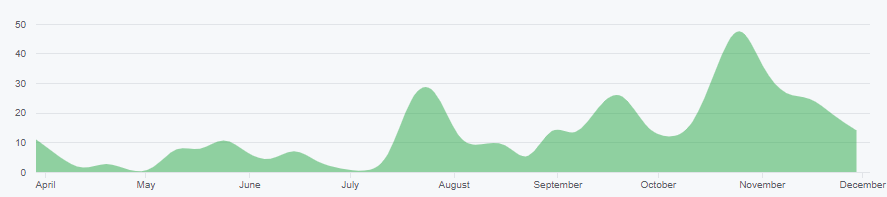
\includegraphics[width=\textwidth]{./resources/commit.png}

而在開發每項功能前,都花了一到兩個星期在做資料搜尋、自學,接著做出最小可行的 Demo,僅僅做出功能還不夠,因為我們做得是遊戲引擎,所以還得將 API 打磨,不斷得去想、擴充功能,因為引擎就是得提供許多功能給遊戲開發者,而在引擎開發階段時,每個功能寫出來之後,還得切換身分到遊戲開發者,試圖用自己做出的引擎來打造遊戲,透過這個過程來除錯和發想可以增加的新功能,一直不斷的迭代,而這個過程是相當漫長和痛苦的,常常在和組員討論時一個功能的規格(spec)時,往往最後都覺得很迷惘,總是覺得這個功能不夠好,但還是得在現實與理想中取捨。

在這次的專案中我也學到了很多東西,像是如何有效與人溝通和合作,表達自己的想法給對方清楚理解,當然過程中勢必有磨合的時期,因為我們是只有四個人的小組,所以作為組長的我理所當然會處理許多工作,也必須擔當起管理的責任,畢竟繁雜的工作量由一個人扛起也過於不切實際,清楚了解到除了程式之外管理和與人相處溝通之道也相當重要。

這個畢業專題算是完成了我其中的一個心願,自幹一個遊戲引擎,也是我目前處理過最多行的程式,算是我的一個小小的里程碑。

% paragraph Roy (end)

\newpage